% 生成最终的图象时把第一个文档类取消注释即可
\documentclass[10pt,varwidth]{standalone}
% \documentclass[12pt]{article}
% 1.必须添加varwidth选项,不然就会报错
\PassOptionsToPackage{quiet}{fontspec}
\usepackage{ctex}
% 必须要保证绘图的纸张足够的大
\usepackage[a4paper, left=2.5cm, right=2.5cm, top=2.5cm, bottom=2.5cm]{geometry}
\usepackage{xifthen}
\usepackage{xfp}
\usepackage{xcolor}
\usepackage{pgfplots}
\usepackage{pgfplotstable}
\pgfplotsset{compat=1.16}
% 2.引用的tikz库
\usetikzlibrary {matrix, chains, trees, decorations}
\usetikzlibrary {arrows.meta, automata,positioning}
\usetikzlibrary {decorations.pathmorphing, calc}
\usetikzlibrary {calligraphy}
\usetikzlibrary {backgrounds, mindmap,shadows}
\usetikzlibrary {patterns, quotes, 3d, shadows}
\usetikzlibrary {graphs, fadings, scopes}
\usetikzlibrary {arrows, shapes.geometric}
\usepgflibrary {shadings}

\tikzset{
    >={Latex}
}



\begin{document}
\centering
\;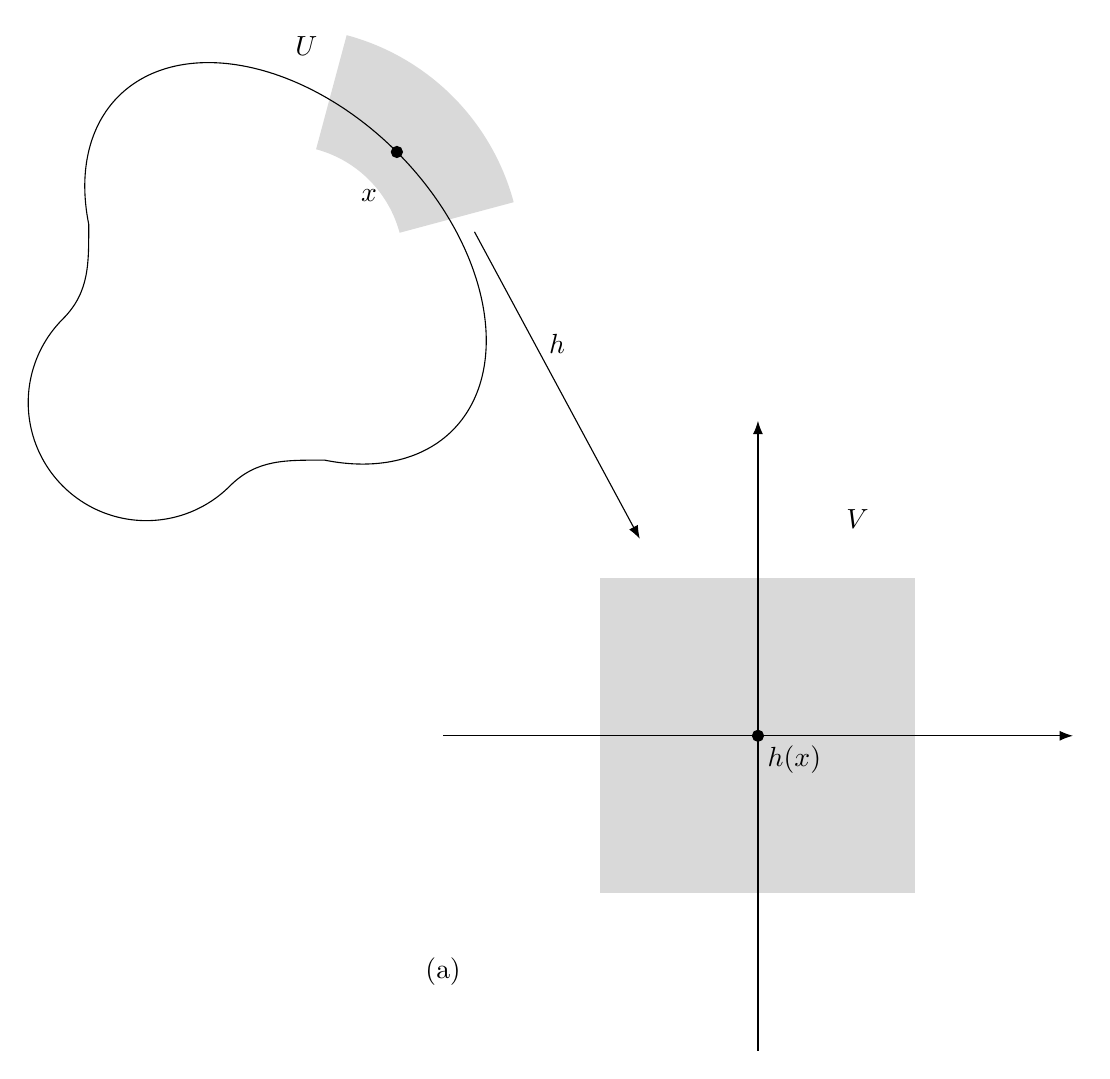
\begin{tikzpicture}
% \draw (-8.06558, 4.19765)
    % to[out=-150, in=45] (-8.87712,3.37946)
    % to[out=-150, in=-30] (-8.6208,2.16714)
    % to[out=-45,  in=30]  (-6.60615,2.10369)
    % to[out=30,   in=-45] (-4.97222,2.26232)
    % to[out=-45,  in=45]  (-3.83006,1.81814)
    % to[out=45,   in=-45] (-4.22664,5.29222)
    % to[out=-45,  in=45]  (-7.1455,5.02255)
    % to[out=45,   in=-150](-8.6208,2.16714);

% upper left
\begin{scope}[xshift=-6cm, yshift=6cm, rotate=-45]
    % fill
    \fill[gray!30] plot[samples=200,domain=60:120,smooth,variable=\t] ({3*cos(\t)}, {3*sin(\t)})
        -- plot[samples=200,domain=120:60,smooth,variable=\t] ({1.5*cos(\t)}, {1.5*sin(\t)})
        -- cycle;
    % frame
    \draw plot[samples=200,domain=-45:225,smooth,variable=\t] ({3*cos(\t)}, {2*sin(\t)});
    \draw plot[samples=200,domain=0:-180,variable=\t] ({1.5*cos(\t)}, {1.5*sin(\t)-2.5});
    \draw (-1.5, -2.5) to[out=90, in=-45] (-2.12, -1.415);
    \draw (1.5, -2.5) to[out=90, in=-135] (2.12, -1.415);
    \node[below] at (90:1.5) {$x$};  
    \node[below right] at (135:3) {$U$};  
    \filldraw (90:2) circle (2pt); 
\end{scope} 
% below right
\begin{scope}
    \fill[gray!30] (-2, -2) -- (2, -2) -- (2, 2) -- (-2, 2) -- cycle;
    \node[below right] at (0, 0) {$h(x)$};  
    \node[below right] at (1, 3) {$V$}; 
    \filldraw (0,0) circle (2pt); 
\end{scope}
% draw xy axis
\draw[->] (-4, 0) -- (4, 0)    node [below] {};
\draw[->] (0, -4)  -- (0, 4)    node [left]  {};
% draw arrow
\draw[->] (-3.6, 6.4) -- (-1.5, 2.5) node[midway, above=8pt] {$h$};
% subfig num
\node at (-4, -3) {(a)};
\end{tikzpicture}
\end{document}